\documentclass[]{article}
\usepackage{lmodern}
\usepackage{amssymb,amsmath}
\usepackage{ifxetex,ifluatex}
\usepackage{fixltx2e} % provides \textsubscript
\ifnum 0\ifxetex 1\fi\ifluatex 1\fi=0 % if pdftex
  \usepackage[T1]{fontenc}
  \usepackage[utf8]{inputenc}
\else % if luatex or xelatex
  \ifxetex
    \usepackage{mathspec}
  \else
    \usepackage{fontspec}
  \fi
  \defaultfontfeatures{Ligatures=TeX,Scale=MatchLowercase}
\fi
% use upquote if available, for straight quotes in verbatim environments
\IfFileExists{upquote.sty}{\usepackage{upquote}}{}
% use microtype if available
\IfFileExists{microtype.sty}{%
\usepackage{microtype}
\UseMicrotypeSet[protrusion]{basicmath} % disable protrusion for tt fonts
}{}
\usepackage[margin=1in]{geometry}
\usepackage{hyperref}
\hypersetup{unicode=true,
            pdftitle={machine learning(732A99) lab2},
            pdfauthor={Anubhav Dikshit(anudi287)},
            pdfborder={0 0 0},
            breaklinks=true}
\urlstyle{same}  % don't use monospace font for urls
\usepackage{color}
\usepackage{fancyvrb}
\newcommand{\VerbBar}{|}
\newcommand{\VERB}{\Verb[commandchars=\\\{\}]}
\DefineVerbatimEnvironment{Highlighting}{Verbatim}{commandchars=\\\{\}}
% Add ',fontsize=\small' for more characters per line
\usepackage{framed}
\definecolor{shadecolor}{RGB}{248,248,248}
\newenvironment{Shaded}{\begin{snugshade}}{\end{snugshade}}
\newcommand{\KeywordTok}[1]{\textcolor[rgb]{0.13,0.29,0.53}{\textbf{#1}}}
\newcommand{\DataTypeTok}[1]{\textcolor[rgb]{0.13,0.29,0.53}{#1}}
\newcommand{\DecValTok}[1]{\textcolor[rgb]{0.00,0.00,0.81}{#1}}
\newcommand{\BaseNTok}[1]{\textcolor[rgb]{0.00,0.00,0.81}{#1}}
\newcommand{\FloatTok}[1]{\textcolor[rgb]{0.00,0.00,0.81}{#1}}
\newcommand{\ConstantTok}[1]{\textcolor[rgb]{0.00,0.00,0.00}{#1}}
\newcommand{\CharTok}[1]{\textcolor[rgb]{0.31,0.60,0.02}{#1}}
\newcommand{\SpecialCharTok}[1]{\textcolor[rgb]{0.00,0.00,0.00}{#1}}
\newcommand{\StringTok}[1]{\textcolor[rgb]{0.31,0.60,0.02}{#1}}
\newcommand{\VerbatimStringTok}[1]{\textcolor[rgb]{0.31,0.60,0.02}{#1}}
\newcommand{\SpecialStringTok}[1]{\textcolor[rgb]{0.31,0.60,0.02}{#1}}
\newcommand{\ImportTok}[1]{#1}
\newcommand{\CommentTok}[1]{\textcolor[rgb]{0.56,0.35,0.01}{\textit{#1}}}
\newcommand{\DocumentationTok}[1]{\textcolor[rgb]{0.56,0.35,0.01}{\textbf{\textit{#1}}}}
\newcommand{\AnnotationTok}[1]{\textcolor[rgb]{0.56,0.35,0.01}{\textbf{\textit{#1}}}}
\newcommand{\CommentVarTok}[1]{\textcolor[rgb]{0.56,0.35,0.01}{\textbf{\textit{#1}}}}
\newcommand{\OtherTok}[1]{\textcolor[rgb]{0.56,0.35,0.01}{#1}}
\newcommand{\FunctionTok}[1]{\textcolor[rgb]{0.00,0.00,0.00}{#1}}
\newcommand{\VariableTok}[1]{\textcolor[rgb]{0.00,0.00,0.00}{#1}}
\newcommand{\ControlFlowTok}[1]{\textcolor[rgb]{0.13,0.29,0.53}{\textbf{#1}}}
\newcommand{\OperatorTok}[1]{\textcolor[rgb]{0.81,0.36,0.00}{\textbf{#1}}}
\newcommand{\BuiltInTok}[1]{#1}
\newcommand{\ExtensionTok}[1]{#1}
\newcommand{\PreprocessorTok}[1]{\textcolor[rgb]{0.56,0.35,0.01}{\textit{#1}}}
\newcommand{\AttributeTok}[1]{\textcolor[rgb]{0.77,0.63,0.00}{#1}}
\newcommand{\RegionMarkerTok}[1]{#1}
\newcommand{\InformationTok}[1]{\textcolor[rgb]{0.56,0.35,0.01}{\textbf{\textit{#1}}}}
\newcommand{\WarningTok}[1]{\textcolor[rgb]{0.56,0.35,0.01}{\textbf{\textit{#1}}}}
\newcommand{\AlertTok}[1]{\textcolor[rgb]{0.94,0.16,0.16}{#1}}
\newcommand{\ErrorTok}[1]{\textcolor[rgb]{0.64,0.00,0.00}{\textbf{#1}}}
\newcommand{\NormalTok}[1]{#1}
\usepackage{graphicx,grffile}
\makeatletter
\def\maxwidth{\ifdim\Gin@nat@width>\linewidth\linewidth\else\Gin@nat@width\fi}
\def\maxheight{\ifdim\Gin@nat@height>\textheight\textheight\else\Gin@nat@height\fi}
\makeatother
% Scale images if necessary, so that they will not overflow the page
% margins by default, and it is still possible to overwrite the defaults
% using explicit options in \includegraphics[width, height, ...]{}
\setkeys{Gin}{width=\maxwidth,height=\maxheight,keepaspectratio}
\IfFileExists{parskip.sty}{%
\usepackage{parskip}
}{% else
\setlength{\parindent}{0pt}
\setlength{\parskip}{6pt plus 2pt minus 1pt}
}
\setlength{\emergencystretch}{3em}  % prevent overfull lines
\providecommand{\tightlist}{%
  \setlength{\itemsep}{0pt}\setlength{\parskip}{0pt}}
\setcounter{secnumdepth}{0}
% Redefines (sub)paragraphs to behave more like sections
\ifx\paragraph\undefined\else
\let\oldparagraph\paragraph
\renewcommand{\paragraph}[1]{\oldparagraph{#1}\mbox{}}
\fi
\ifx\subparagraph\undefined\else
\let\oldsubparagraph\subparagraph
\renewcommand{\subparagraph}[1]{\oldsubparagraph{#1}\mbox{}}
\fi

%%% Use protect on footnotes to avoid problems with footnotes in titles
\let\rmarkdownfootnote\footnote%
\def\footnote{\protect\rmarkdownfootnote}

%%% Change title format to be more compact
\usepackage{titling}

% Create subtitle command for use in maketitle
\newcommand{\subtitle}[1]{
  \posttitle{
    \begin{center}\large#1\end{center}
    }
}

\setlength{\droptitle}{-2em}

  \title{machine learning(732A99) lab2}
    \pretitle{\vspace{\droptitle}\centering\huge}
  \posttitle{\par}
    \author{Anubhav Dikshit(anudi287)}
    \preauthor{\centering\large\emph}
  \postauthor{\par}
      \predate{\centering\large\emph}
  \postdate{\par}
    \date{10 December 2018}


\begin{document}
\maketitle

{
\setcounter{tocdepth}{2}
\tableofcontents
}
\newpage

\section{Assignment 1}\label{assignment-1}

\subsection{Loading The Libraries}\label{loading-the-libraries}

\subsection{Loading Input files}\label{loading-input-files}

\begin{Shaded}
\begin{Highlighting}[]
\NormalTok{crab_data <-}\StringTok{ }\KeywordTok{read.csv}\NormalTok{(}\DataTypeTok{file =} \StringTok{"australian-crabs.csv"}\NormalTok{, }\DataTypeTok{header =} \OtherTok{TRUE}\NormalTok{)}
\NormalTok{credit_data <-}\StringTok{ }\KeywordTok{read.xlsx}\NormalTok{(}\StringTok{"creditscoring.xls"}\NormalTok{, }\DataTypeTok{sheetName =} \StringTok{"credit"}\NormalTok{)}
\end{Highlighting}
\end{Shaded}

\subsection{1.1 Use australian-crabs.csv and make a scatterplot of
carapace length (CL) versus rear width (RW) where observations are
colored by Sex. Do you think that this data is easy to classify by
linear discriminant analysis? Motivate your
answer.}\label{use-australian-crabs.csv-and-make-a-scatterplot-of-carapace-length-cl-versus-rear-width-rw-where-observations-are-colored-by-sex.-do-you-think-that-this-data-is-easy-to-classify-by-linear-discriminant-analysis-motivate-your-answer.}

\begin{Shaded}
\begin{Highlighting}[]
\NormalTok{p1 <-}\StringTok{ }\KeywordTok{ggplot}\NormalTok{(}\DataTypeTok{data =}\NormalTok{ crab_data, }\KeywordTok{aes}\NormalTok{(}\DataTypeTok{x =}\NormalTok{ CL, }\DataTypeTok{y =}\NormalTok{ RW, }\DataTypeTok{color =}\NormalTok{ sex )) }\OperatorTok{+}\StringTok{ }\KeywordTok{geom_point}\NormalTok{() }\OperatorTok{+}\StringTok{ }
\StringTok{  }\KeywordTok{geom_smooth}\NormalTok{(}\DataTypeTok{method =} \StringTok{'loess'}\NormalTok{) }\OperatorTok{+}\StringTok{ }
\StringTok{  }\KeywordTok{ggtitle}\NormalTok{(}\StringTok{"Scatter Plot of Carapace Length vs. Rear Width by Sex"}\NormalTok{)}

\NormalTok{mu_CL <-}\StringTok{ }\NormalTok{crab_data }\OperatorTok\StringTok{ }
\StringTok{  }\KeywordTok{group_by}\NormalTok{(sex) }\OperatorTok
\StringTok{  }\KeywordTok{summarise}\NormalTok{(}\DataTypeTok{grp.mean =} \KeywordTok{mean}\NormalTok{(CL))}

\NormalTok{mu_RW <-}\StringTok{ }\NormalTok{crab_data }\OperatorTok\StringTok{ }
\StringTok{  }\KeywordTok{group_by}\NormalTok{(sex) }\OperatorTok
\StringTok{  }\KeywordTok{summarise}\NormalTok{(}\DataTypeTok{grp.mean =} \KeywordTok{mean}\NormalTok{(RW))}


\KeywordTok{ggplot}\NormalTok{(}\DataTypeTok{data =}\NormalTok{ crab_data, }\KeywordTok{aes}\NormalTok{(}\DataTypeTok{x =}\NormalTok{ CL)) }\OperatorTok{+}\StringTok{ }
\StringTok{  }\KeywordTok{geom_density}\NormalTok{(}\KeywordTok{aes}\NormalTok{(}\DataTypeTok{fill =}\NormalTok{ sex), }\DataTypeTok{alpha =} \FloatTok{0.3}\NormalTok{) }\OperatorTok{+}
\StringTok{      }\KeywordTok{geom_vline}\NormalTok{(}\KeywordTok{aes}\NormalTok{(}\DataTypeTok{xintercept =}\NormalTok{ grp.mean, }\DataTypeTok{color =}\NormalTok{ sex), }
                 \DataTypeTok{data =}\NormalTok{ mu_CL, }\DataTypeTok{linetype =} \StringTok{"dashed"}\NormalTok{) }\OperatorTok{+}\StringTok{ }
\StringTok{  }\KeywordTok{ggtitle}\NormalTok{(}\StringTok{"Density plot of Carapace Length vs. gender"}\NormalTok{)}
\end{Highlighting}
\end{Shaded}

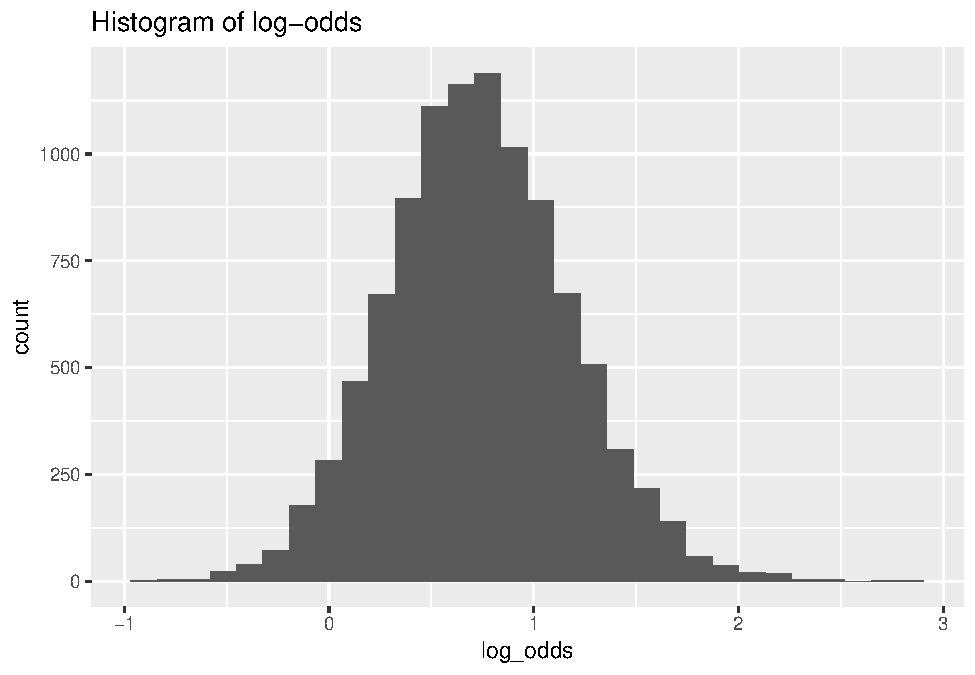
\includegraphics{machine_learning_lab2_files/figure-latex/unnamed-chunk-3-1.pdf}

\begin{Shaded}
\begin{Highlighting}[]
\KeywordTok{ggplot}\NormalTok{(}\DataTypeTok{data =}\NormalTok{ crab_data, }\KeywordTok{aes}\NormalTok{(}\DataTypeTok{x =}\NormalTok{ RW)) }\OperatorTok{+}\StringTok{ }
\StringTok{  }\KeywordTok{geom_density}\NormalTok{(}\KeywordTok{aes}\NormalTok{(}\DataTypeTok{fill =}\NormalTok{ sex), }\DataTypeTok{alpha =} \FloatTok{0.3}\NormalTok{) }\OperatorTok{+}
\StringTok{      }\KeywordTok{geom_vline}\NormalTok{(}\KeywordTok{aes}\NormalTok{(}\DataTypeTok{xintercept =}\NormalTok{ grp.mean, }\DataTypeTok{color =}\NormalTok{ sex),}
             \DataTypeTok{data =}\NormalTok{ mu_RW, }\DataTypeTok{linetype =} \StringTok{"dashed"}\NormalTok{) }\OperatorTok{+}\StringTok{ }
\StringTok{  }\KeywordTok{ggtitle}\NormalTok{(}\StringTok{"Density plot of Rear Width vs. gender"}\NormalTok{)}
\end{Highlighting}
\end{Shaded}

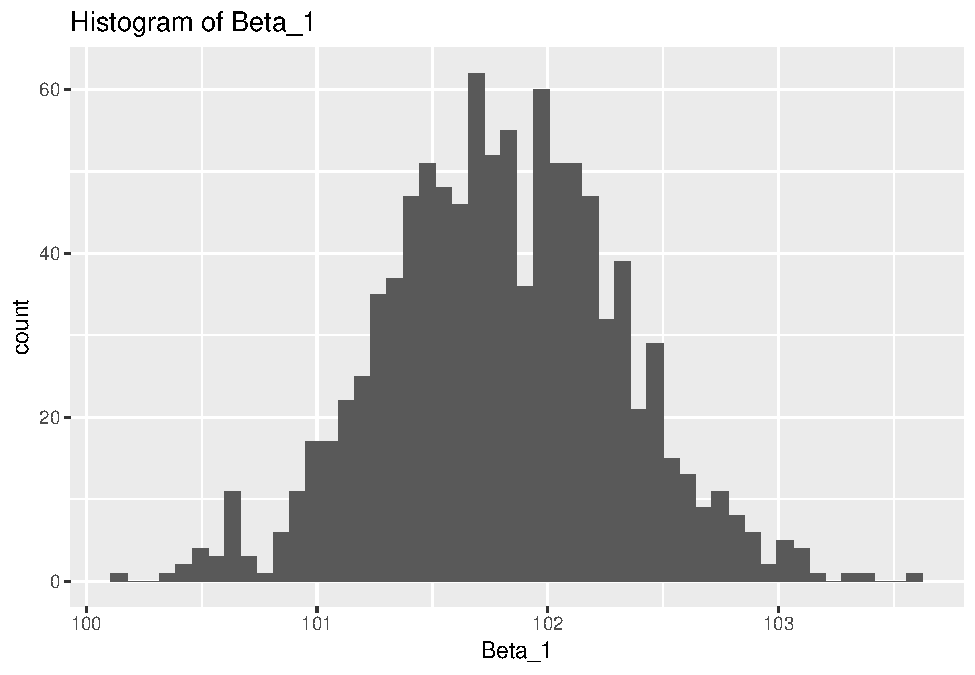
\includegraphics{machine_learning_lab2_files/figure-latex/unnamed-chunk-3-2.pdf}

Analysis: In Linear Discriminant Analysis (LDA) the boundary between
differenet class of datapoints is a line just as the case in a logistics
regression. In LDA there is an assumption that the data points for each
class come from a Gaussian distribution with same variance,but different
means, just as an added measure we have plotted this also. Here we find
that for variable `Carapace Length' the mean is only slightly different
however for variable `Rear width' the mean between the two sex is
seperated by a larger margin.

Thus although the assumptions are violated a bit, judging by the orginal
scatter plot we do find this to be case where LDA might do a good job.

\subsection{1.2 Make LDA analysis with target Sex and features CL and RW
and proportional prior by using lda() function in package MASS. Make a
scatter plot of CL versus RW colored by the predicted Sex and compare it
with the plot in step 1. Compute the misclassification error and comment
on the quality of
fit.}\label{make-lda-analysis-with-target-sex-and-features-cl-and-rw-and-proportional-prior-by-using-lda-function-in-package-mass.-make-a-scatter-plot-of-cl-versus-rw-colored-by-the-predicted-sex-and-compare-it-with-the-plot-in-step-1.-compute-the-misclassification-error-and-comment-on-the-quality-of-fit.}

\begin{Shaded}
\begin{Highlighting}[]
\KeywordTok{set.seed}\NormalTok{(}\DecValTok{12345}\NormalTok{)}
\NormalTok{temp <-}\StringTok{ }\NormalTok{crab_data}

\NormalTok{## using priors same as the propotional of the dataset}
\NormalTok{crab_lda <-}\StringTok{ }\NormalTok{MASS}\OperatorTok{::}\KeywordTok{lda}\NormalTok{(}\DataTypeTok{formula =}\NormalTok{ sex }\OperatorTok{~}\StringTok{ }\NormalTok{CL}\OperatorTok{+}\StringTok{ }\NormalTok{RW, }\DataTypeTok{data =}\NormalTok{ temp)}
\KeywordTok{print}\NormalTok{(crab_lda)}
\end{Highlighting}
\end{Shaded}

\begin{verbatim}
## Call:
## lda(sex ~ CL + RW, data = temp)
## 
## Prior probabilities of groups:
## Female   Male 
##    0.5    0.5 
## 
## Group means:
##            CL     RW
## Female 31.360 13.487
## Male   32.851 11.990
## 
## Coefficients of linear discriminants:
##           LD1
## CL  0.5765241
## RW -1.6823062
\end{verbatim}

\begin{Shaded}
\begin{Highlighting}[]
\NormalTok{lda_predicted_class <-}\StringTok{ }\KeywordTok{predict}\NormalTok{(crab_lda, }\DataTypeTok{newdata =}\NormalTok{ temp)}
\NormalTok{temp}\OperatorTok{$}\NormalTok{lda_predicted_sex <-}\StringTok{ }\NormalTok{lda_predicted_class}\OperatorTok{$}\NormalTok{class}

\NormalTok{p2 <-}\StringTok{ }\KeywordTok{ggplot}\NormalTok{(}\DataTypeTok{data =}\NormalTok{ temp, }\KeywordTok{aes}\NormalTok{(}\DataTypeTok{x =}\NormalTok{ CL, }\DataTypeTok{y =}\NormalTok{ RW, }\DataTypeTok{color =}\NormalTok{ lda_predicted_sex)) }\OperatorTok{+}\StringTok{ }
\StringTok{  }\KeywordTok{geom_point}\NormalTok{() }\OperatorTok{+}\StringTok{ }\KeywordTok{geom_smooth}\NormalTok{(}\DataTypeTok{method =} \StringTok{'loess'}\NormalTok{) }\OperatorTok{+}\StringTok{ }
\StringTok{  }\KeywordTok{ggtitle}\NormalTok{(}\StringTok{"Scatter Plot of Carapace Length vs. Rear Width by Predicted Sex"}\NormalTok{)}

\NormalTok{gridExtra}\OperatorTok{::}\KeywordTok{grid.arrange}\NormalTok{(p1, p2, }\DataTypeTok{nrow =} \DecValTok{2}\NormalTok{)}
\end{Highlighting}
\end{Shaded}

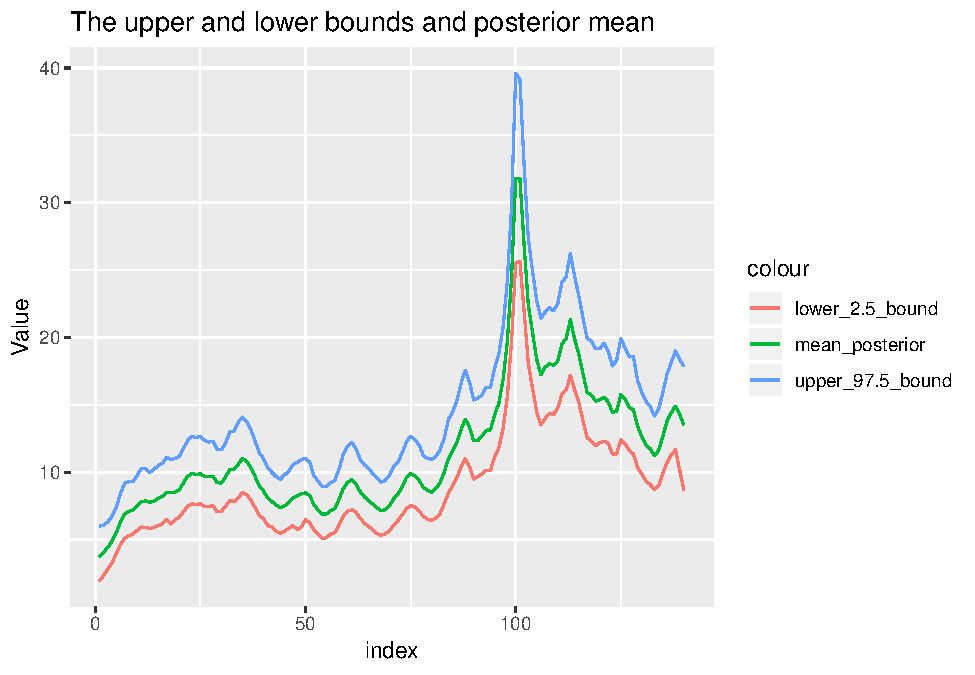
\includegraphics{machine_learning_lab2_files/figure-latex/unnamed-chunk-4-1.pdf}

\begin{Shaded}
\begin{Highlighting}[]
\NormalTok{misclassification_lda <-}\StringTok{ }\KeywordTok{table}\NormalTok{(temp}\OperatorTok{$}\NormalTok{sex, temp}\OperatorTok{$}\NormalTok{lda_predicted_sex)}
\KeywordTok{names}\NormalTok{(}\KeywordTok{dimnames}\NormalTok{(misclassification_lda)) <-}\StringTok{ }\KeywordTok{c}\NormalTok{(}\StringTok{"Actual"}\NormalTok{, }\StringTok{"Predicted"}\NormalTok{)}
\NormalTok{caret}\OperatorTok{::}\KeywordTok{confusionMatrix}\NormalTok{(misclassification_lda)}
\end{Highlighting}
\end{Shaded}

\begin{verbatim}
## Confusion Matrix and Statistics
## 
##         Predicted
## Actual   Female Male
##   Female     97    3
##   Male        4   96
##                                              
##                Accuracy : 0.965              
##                  95% CI : (0.9292, 0.9858)   
##     No Information Rate : 0.505              
##     P-Value [Acc > NIR] : <0.0000000000000002
##                                              
##                   Kappa : 0.93               
##  Mcnemar's Test P-Value : 1                  
##                                              
##             Sensitivity : 0.9604             
##             Specificity : 0.9697             
##          Pos Pred Value : 0.9700             
##          Neg Pred Value : 0.9600             
##              Prevalence : 0.5050             
##          Detection Rate : 0.4850             
##    Detection Prevalence : 0.5000             
##       Balanced Accuracy : 0.9650             
##                                              
##        'Positive' Class : Female             
## 
\end{verbatim}

Analysis:

The Accuracy of the fit is 96.5\% thus the misclassification rate is
3.5\%. Such a high value suggests that our model maybe overfit on the
dataset, however to asses the fit we need a test dataset.

As evident from the plot we see that some of `Female' crabs are
classified as `Males' especially when the Carapace Length (CL) is below
20 and Rear width(RW) is below 10.

\subsection{1.3 Repeat step 2 but use priors p(Male)=0.9, p(Female)=0.1
instead. How did the classification result change and
why?}\label{repeat-step-2-but-use-priors-pmale0.9-pfemale0.1-instead.-how-did-the-classification-result-change-and-why}

\begin{Shaded}
\begin{Highlighting}[]
\KeywordTok{set.seed}\NormalTok{(}\DecValTok{12345}\NormalTok{)}
\NormalTok{temp <-}\StringTok{ }\NormalTok{crab_data}

\NormalTok{## using priors same as the propotional of the dataset}
\NormalTok{crab_lda <-}\StringTok{ }\NormalTok{MASS}\OperatorTok{::}\KeywordTok{lda}\NormalTok{(}\DataTypeTok{formula =}\NormalTok{ sex }\OperatorTok{~}\StringTok{ }\NormalTok{CL}\OperatorTok{+}\StringTok{ }\NormalTok{RW, }\DataTypeTok{data =}\NormalTok{ temp, }\DataTypeTok{prior =} \KeywordTok{c}\NormalTok{(}\FloatTok{0.1}\NormalTok{, }\FloatTok{0.9}\NormalTok{))}
\KeywordTok{print}\NormalTok{(crab_lda)}
\end{Highlighting}
\end{Shaded}

\begin{verbatim}
## Call:
## lda(sex ~ CL + RW, data = temp, prior = c(0.1, 0.9))
## 
## Prior probabilities of groups:
## Female   Male 
##    0.1    0.9 
## 
## Group means:
##            CL     RW
## Female 31.360 13.487
## Male   32.851 11.990
## 
## Coefficients of linear discriminants:
##           LD1
## CL  0.5765241
## RW -1.6823062
\end{verbatim}

\begin{Shaded}
\begin{Highlighting}[]
\NormalTok{lda_predicted_class <-}\StringTok{ }\KeywordTok{predict}\NormalTok{(crab_lda, }\DataTypeTok{newdata =}\NormalTok{ temp)}
\NormalTok{temp}\OperatorTok{$}\NormalTok{lda_predicted_sex <-}\StringTok{ }\NormalTok{lda_predicted_class}\OperatorTok{$}\NormalTok{class}

\NormalTok{p3 <-}\StringTok{ }\KeywordTok{ggplot}\NormalTok{(}\DataTypeTok{data =}\NormalTok{ temp, }\KeywordTok{aes}\NormalTok{(}\DataTypeTok{x =}\NormalTok{ CL, }\DataTypeTok{y =}\NormalTok{ RW, }\DataTypeTok{color =}\NormalTok{ lda_predicted_sex)) }\OperatorTok{+}\StringTok{ }
\StringTok{  }\KeywordTok{geom_point}\NormalTok{() }\OperatorTok{+}\StringTok{ }\KeywordTok{geom_smooth}\NormalTok{(}\DataTypeTok{method =} \StringTok{'loess'}\NormalTok{) }\OperatorTok{+}\StringTok{ }
\StringTok{  }\KeywordTok{ggtitle}\NormalTok{(}\StringTok{"Scatter Plot of Carapace Length vs. Rear Width by Predicted Sex(Prior changed)"}\NormalTok{)}

\NormalTok{gridExtra}\OperatorTok{::}\KeywordTok{grid.arrange}\NormalTok{(p2, p3, }\DataTypeTok{nrow =} \DecValTok{2}\NormalTok{)}
\end{Highlighting}
\end{Shaded}

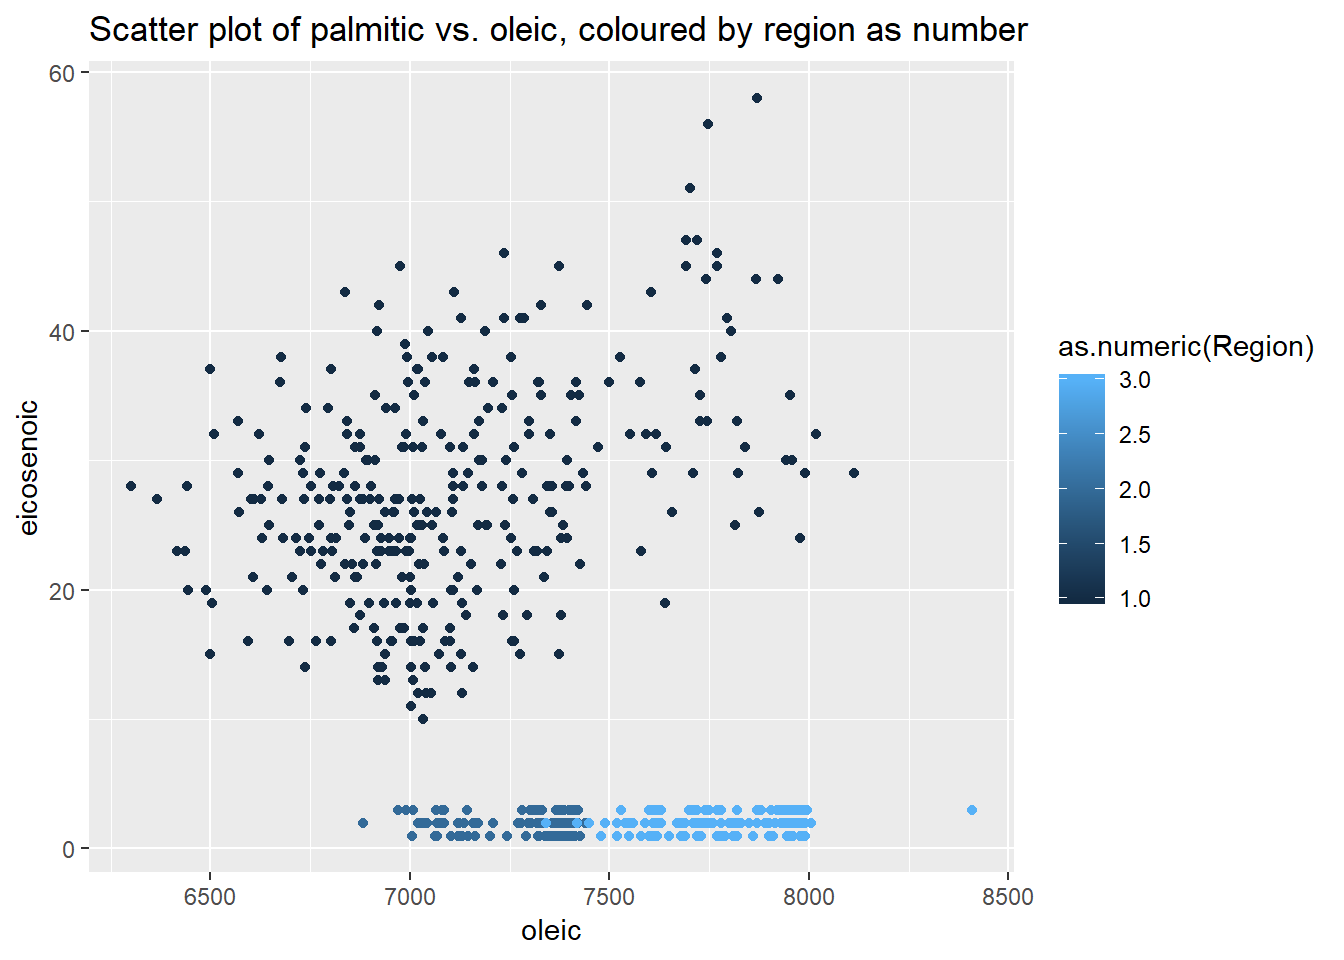
\includegraphics{machine_learning_lab2_files/figure-latex/unnamed-chunk-5-1.pdf}

\begin{Shaded}
\begin{Highlighting}[]
\NormalTok{misclassification_lda <-}\StringTok{ }\KeywordTok{table}\NormalTok{(temp}\OperatorTok{$}\NormalTok{sex, temp}\OperatorTok{$}\NormalTok{lda_predicted_sex)}
\KeywordTok{names}\NormalTok{(}\KeywordTok{dimnames}\NormalTok{(misclassification_lda)) <-}\StringTok{ }\KeywordTok{c}\NormalTok{(}\StringTok{"Actual"}\NormalTok{, }\StringTok{"Predicted"}\NormalTok{)}
\NormalTok{caret}\OperatorTok{::}\KeywordTok{confusionMatrix}\NormalTok{(misclassification_lda)}
\end{Highlighting}
\end{Shaded}

\begin{verbatim}
## Confusion Matrix and Statistics
## 
##         Predicted
## Actual   Female Male
##   Female     84   16
##   Male        0  100
##                                                
##                Accuracy : 0.92                 
##                  95% CI : (0.8733, 0.9536)     
##     No Information Rate : 0.58                 
##     P-Value [Acc > NIR] : < 0.00000000000000022
##                                                
##                   Kappa : 0.84                 
##  Mcnemar's Test P-Value : 0.0001768            
##                                                
##             Sensitivity : 1.0000               
##             Specificity : 0.8621               
##          Pos Pred Value : 0.8400               
##          Neg Pred Value : 1.0000               
##              Prevalence : 0.4200               
##          Detection Rate : 0.4200               
##    Detection Prevalence : 0.5000               
##       Balanced Accuracy : 0.9310               
##                                                
##        'Positive' Class : Female               
## 
\end{verbatim}

Analysis:

The Accuracy of the fit is 92\% thus the misclassification rate is 8\%.

As evident from the confusion matrix we notice that all `Males' crabs
are classfied correctly, while some (16/100) of the female crabs are
classified wrongly.

Compared to previous plot we see that the extend of misclassification
for females has increased for lower values of CW and RL compared to
previous model with prior same as the dataset.

The classification is worse now compared to previous model because the
dataset has the priors of 50-50 for both the sexes while we biased the
model with wrong prior.

\subsection{1.4 Make a similar kind of classification by logistic
regression (use function glm()), plot the classified data and compute
the misclassification error. Compare these results with the LDA results.
Finally, report the equation of the decision boundary and draw it in the
plot of the classified
data.}\label{make-a-similar-kind-of-classification-by-logistic-regression-use-function-glm-plot-the-classified-data-and-compute-the-misclassification-error.-compare-these-results-with-the-lda-results.-finally-report-the-equation-of-the-decision-boundary-and-draw-it-in-the-plot-of-the-classified-data.}

\begin{Shaded}
\begin{Highlighting}[]
\KeywordTok{set.seed}\NormalTok{(}\DecValTok{12345}\NormalTok{)}
\NormalTok{temp <-}\StringTok{ }\NormalTok{crab_data}

\NormalTok{## using priors same as the propotional of the dataset}
\NormalTok{crab_logit <-}\StringTok{ }\KeywordTok{glm}\NormalTok{(}\DataTypeTok{formula =}\NormalTok{ sex }\OperatorTok{~}\StringTok{ }\NormalTok{CL}\OperatorTok{+}\StringTok{ }\NormalTok{RW, }\DataTypeTok{data =}\NormalTok{ temp, }\DataTypeTok{family =}\NormalTok{ binomial)}
\KeywordTok{summary}\NormalTok{(crab_logit)}
\end{Highlighting}
\end{Shaded}

\begin{verbatim}
## 
## Call:
## glm(formula = sex ~ CL + RW, family = binomial, data = temp)
## 
## Deviance Residuals: 
##      Min        1Q    Median        3Q       Max  
## -1.85416  -0.00700   0.00000   0.00081   1.89302  
## 
## Coefficients:
##             Estimate Std. Error z value Pr(>|z|)    
## (Intercept)   13.617      4.251   3.203 0.001359 ** 
## CL             4.631      1.352   3.426 0.000612 ***
## RW           -12.564      3.611  -3.479 0.000503 ***
## ---
## Signif. codes:  0 '***' 0.001 '**' 0.01 '*' 0.05 '.' 0.1 ' ' 1
## 
## (Dispersion parameter for binomial family taken to be 1)
## 
##     Null deviance: 277.259  on 199  degrees of freedom
## Residual deviance:  24.095  on 197  degrees of freedom
## AIC: 30.095
## 
## Number of Fisher Scoring iterations: 10
\end{verbatim}

\begin{Shaded}
\begin{Highlighting}[]
\NormalTok{logit_predicted_class <-}\StringTok{ }\KeywordTok{predict}\NormalTok{(crab_logit, }\DataTypeTok{newdata =}\NormalTok{ temp, }\DataTypeTok{type =} \KeywordTok{c}\NormalTok{(}\StringTok{"response"}\NormalTok{))}
\NormalTok{temp}\OperatorTok{$}\NormalTok{logit_predicted_prob <-}\StringTok{ }\NormalTok{logit_predicted_class}
\NormalTok{temp}\OperatorTok{$}\NormalTok{logit_predicted_sex <-}\StringTok{ }\KeywordTok{ifelse}\NormalTok{(temp}\OperatorTok{$}\NormalTok{logit_predicted_prob }\OperatorTok{>=}\StringTok{ }\FloatTok{0.5}\NormalTok{, }\StringTok{"Male"}\NormalTok{, }\StringTok{"Female"}\NormalTok{)}

\NormalTok{p4 <-}\StringTok{ }\KeywordTok{ggplot}\NormalTok{(}\DataTypeTok{data =}\NormalTok{ temp, }\KeywordTok{aes}\NormalTok{(}\DataTypeTok{x =}\NormalTok{ CL, }\DataTypeTok{y =}\NormalTok{ RW, }\DataTypeTok{color =}\NormalTok{ logit_predicted_sex)) }\OperatorTok{+}\StringTok{ }
\StringTok{  }\KeywordTok{geom_point}\NormalTok{() }\OperatorTok{+}\StringTok{ }\KeywordTok{geom_smooth}\NormalTok{(}\DataTypeTok{method =} \StringTok{'loess'}\NormalTok{) }\OperatorTok{+}\StringTok{ }
\StringTok{  }\KeywordTok{ggtitle}\NormalTok{(}\StringTok{"Scatter Plot of Carapace Length vs. Rear Width by Predicted Sex(Logit)"}\NormalTok{)}

\NormalTok{gridExtra}\OperatorTok{::}\KeywordTok{grid.arrange}\NormalTok{(p3, p4, }\DataTypeTok{nrow =} \DecValTok{2}\NormalTok{)}
\end{Highlighting}
\end{Shaded}

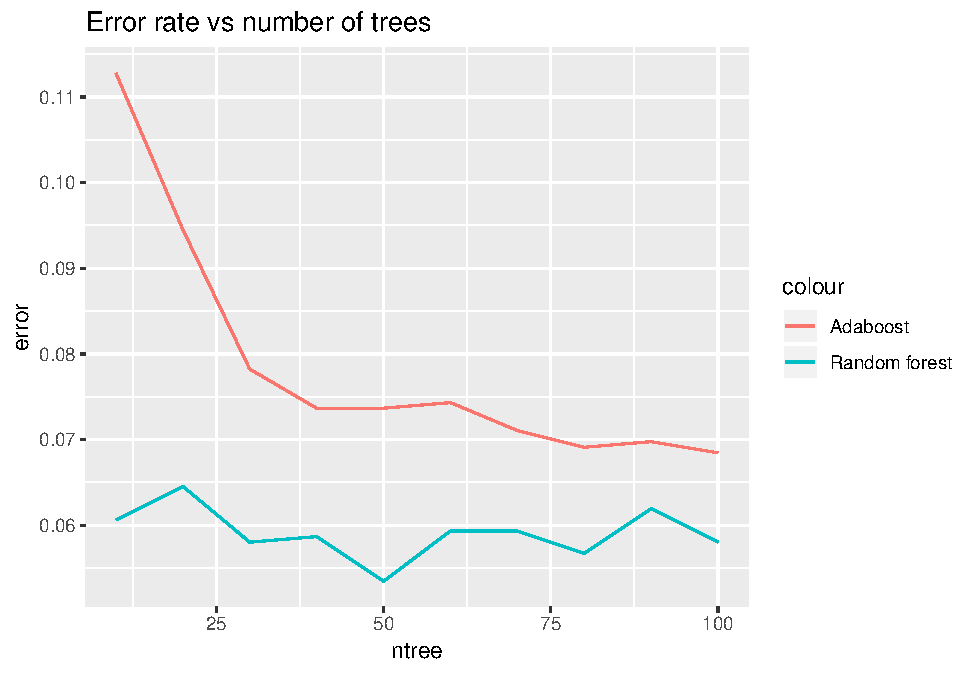
\includegraphics{machine_learning_lab2_files/figure-latex/unnamed-chunk-6-1.pdf}

\begin{Shaded}
\begin{Highlighting}[]
\NormalTok{misclassification_logit <-}\StringTok{ }\KeywordTok{table}\NormalTok{(temp}\OperatorTok{$}\NormalTok{sex, temp}\OperatorTok{$}\NormalTok{logit_predicted_sex)}
\KeywordTok{names}\NormalTok{(}\KeywordTok{dimnames}\NormalTok{(misclassification_logit)) <-}\StringTok{ }\KeywordTok{c}\NormalTok{(}\StringTok{"Actual"}\NormalTok{, }\StringTok{"Predicted"}\NormalTok{)}
\NormalTok{caret}\OperatorTok{::}\KeywordTok{confusionMatrix}\NormalTok{(misclassification_logit)}
\end{Highlighting}
\end{Shaded}

\begin{verbatim}
## Confusion Matrix and Statistics
## 
##         Predicted
## Actual   Female Male
##   Female     97    3
##   Male        4   96
##                                              
##                Accuracy : 0.965              
##                  95% CI : (0.9292, 0.9858)   
##     No Information Rate : 0.505              
##     P-Value [Acc > NIR] : <0.0000000000000002
##                                              
##                   Kappa : 0.93               
##  Mcnemar's Test P-Value : 1                  
##                                              
##             Sensitivity : 0.9604             
##             Specificity : 0.9697             
##          Pos Pred Value : 0.9700             
##          Neg Pred Value : 0.9600             
##              Prevalence : 0.5050             
##          Detection Rate : 0.4850             
##    Detection Prevalence : 0.5000             
##       Balanced Accuracy : 0.9650             
##                                              
##        'Positive' Class : Female             
## 
\end{verbatim}

\begin{Shaded}
\begin{Highlighting}[]
\KeywordTok{ggplot}\NormalTok{(crab_logit, }\KeywordTok{aes}\NormalTok{(}\DataTypeTok{x =}\NormalTok{ CL, }\DataTypeTok{y =}\NormalTok{ RW)) }\OperatorTok{+}\StringTok{ }
\StringTok{  }\KeywordTok{geom_line}\NormalTok{() }\OperatorTok{+}\StringTok{  }
\StringTok{  }\KeywordTok{ggtitle}\NormalTok{(}\StringTok{"Decision boundary"}\NormalTok{)}
\end{Highlighting}
\end{Shaded}

\includegraphics{machine_learning_lab2_files/figure-latex/unnamed-chunk-6-2.pdf}

\tiny{Pr}(\text{Vote} = 1 \textbar{} \text{S, P, I}) \&=
\textbackslash{}frac\{\text{exp}(\beta\_0 + \beta\_1 \text{Gender} +
\beta\_2

\section{Appendix}\label{appendix}

\begin{Shaded}
\begin{Highlighting}[]
\NormalTok{knitr}\OperatorTok{::}\NormalTok{opts_chunk}\OperatorTok{$}\KeywordTok{set}\NormalTok{(}\DataTypeTok{echo =} \OtherTok{TRUE}\NormalTok{)}
\ControlFlowTok{if}\NormalTok{ (}\OperatorTok{!}\KeywordTok{require}\NormalTok{(}\StringTok{"pacman"}\NormalTok{)) }\KeywordTok{install.packages}\NormalTok{(}\StringTok{"pacman"}\NormalTok{)}
\NormalTok{pacman}\OperatorTok{::}\KeywordTok{p_load}\NormalTok{(xlsx, ggplot2, MASS, tidyr, dplyr, reshape2, gridExtra)}

\KeywordTok{set.seed}\NormalTok{(}\DecValTok{12345}\NormalTok{)}
\KeywordTok{options}\NormalTok{(}\StringTok{"jtools-digits"}\NormalTok{ =}\StringTok{ }\DecValTok{2}\NormalTok{, }\DataTypeTok{scipen =} \DecValTok{999}\NormalTok{)}
\NormalTok{crab_data <-}\StringTok{ }\KeywordTok{read.csv}\NormalTok{(}\DataTypeTok{file =} \StringTok{"australian-crabs.csv"}\NormalTok{, }\DataTypeTok{header =} \OtherTok{TRUE}\NormalTok{)}
\NormalTok{credit_data <-}\StringTok{ }\KeywordTok{read.xlsx}\NormalTok{(}\StringTok{"creditscoring.xls"}\NormalTok{, }\DataTypeTok{sheetName =} \StringTok{"credit"}\NormalTok{)}
\NormalTok{p1 <-}\StringTok{ }\KeywordTok{ggplot}\NormalTok{(}\DataTypeTok{data =}\NormalTok{ crab_data, }\KeywordTok{aes}\NormalTok{(}\DataTypeTok{x =}\NormalTok{ CL, }\DataTypeTok{y =}\NormalTok{ RW, }\DataTypeTok{color =}\NormalTok{ sex )) }\OperatorTok{+}\StringTok{ }\KeywordTok{geom_point}\NormalTok{() }\OperatorTok{+}\StringTok{ }
\StringTok{  }\KeywordTok{geom_smooth}\NormalTok{(}\DataTypeTok{method =} \StringTok{'loess'}\NormalTok{) }\OperatorTok{+}\StringTok{ }
\StringTok{  }\KeywordTok{ggtitle}\NormalTok{(}\StringTok{"Scatter Plot of Carapace Length vs. Rear Width by Sex"}\NormalTok{)}

\NormalTok{mu_CL <-}\StringTok{ }\NormalTok{crab_data }\OperatorTok\StringTok{ }
\StringTok{  }\KeywordTok{group_by}\NormalTok{(sex) }\OperatorTok
\StringTok{  }\KeywordTok{summarise}\NormalTok{(}\DataTypeTok{grp.mean =} \KeywordTok{mean}\NormalTok{(CL))}

\NormalTok{mu_RW <-}\StringTok{ }\NormalTok{crab_data }\OperatorTok\StringTok{ }
\StringTok{  }\KeywordTok{group_by}\NormalTok{(sex) }\OperatorTok
\StringTok{  }\KeywordTok{summarise}\NormalTok{(}\DataTypeTok{grp.mean =} \KeywordTok{mean}\NormalTok{(RW))}


\KeywordTok{ggplot}\NormalTok{(}\DataTypeTok{data =}\NormalTok{ crab_data, }\KeywordTok{aes}\NormalTok{(}\DataTypeTok{x =}\NormalTok{ CL)) }\OperatorTok{+}\StringTok{ }
\StringTok{  }\KeywordTok{geom_density}\NormalTok{(}\KeywordTok{aes}\NormalTok{(}\DataTypeTok{fill =}\NormalTok{ sex), }\DataTypeTok{alpha =} \FloatTok{0.3}\NormalTok{) }\OperatorTok{+}
\StringTok{      }\KeywordTok{geom_vline}\NormalTok{(}\KeywordTok{aes}\NormalTok{(}\DataTypeTok{xintercept =}\NormalTok{ grp.mean, }\DataTypeTok{color =}\NormalTok{ sex), }
                 \DataTypeTok{data =}\NormalTok{ mu_CL, }\DataTypeTok{linetype =} \StringTok{"dashed"}\NormalTok{) }\OperatorTok{+}\StringTok{ }
\StringTok{  }\KeywordTok{ggtitle}\NormalTok{(}\StringTok{"Density plot of Carapace Length vs. gender"}\NormalTok{)}


\KeywordTok{ggplot}\NormalTok{(}\DataTypeTok{data =}\NormalTok{ crab_data, }\KeywordTok{aes}\NormalTok{(}\DataTypeTok{x =}\NormalTok{ RW)) }\OperatorTok{+}\StringTok{ }
\StringTok{  }\KeywordTok{geom_density}\NormalTok{(}\KeywordTok{aes}\NormalTok{(}\DataTypeTok{fill =}\NormalTok{ sex), }\DataTypeTok{alpha =} \FloatTok{0.3}\NormalTok{) }\OperatorTok{+}
\StringTok{      }\KeywordTok{geom_vline}\NormalTok{(}\KeywordTok{aes}\NormalTok{(}\DataTypeTok{xintercept =}\NormalTok{ grp.mean, }\DataTypeTok{color =}\NormalTok{ sex),}
             \DataTypeTok{data =}\NormalTok{ mu_RW, }\DataTypeTok{linetype =} \StringTok{"dashed"}\NormalTok{) }\OperatorTok{+}\StringTok{ }
\StringTok{  }\KeywordTok{ggtitle}\NormalTok{(}\StringTok{"Density plot of Rear Width vs. gender"}\NormalTok{)}


\KeywordTok{set.seed}\NormalTok{(}\DecValTok{12345}\NormalTok{)}
\NormalTok{temp <-}\StringTok{ }\NormalTok{crab_data}

\NormalTok{## using priors same as the propotional of the dataset}
\NormalTok{crab_lda <-}\StringTok{ }\NormalTok{MASS}\OperatorTok{::}\KeywordTok{lda}\NormalTok{(}\DataTypeTok{formula =}\NormalTok{ sex }\OperatorTok{~}\StringTok{ }\NormalTok{CL}\OperatorTok{+}\StringTok{ }\NormalTok{RW, }\DataTypeTok{data =}\NormalTok{ temp)}
\KeywordTok{print}\NormalTok{(crab_lda)}

\NormalTok{lda_predicted_class <-}\StringTok{ }\KeywordTok{predict}\NormalTok{(crab_lda, }\DataTypeTok{newdata =}\NormalTok{ temp)}
\NormalTok{temp}\OperatorTok{$}\NormalTok{lda_predicted_sex <-}\StringTok{ }\NormalTok{lda_predicted_class}\OperatorTok{$}\NormalTok{class}

\NormalTok{p2 <-}\StringTok{ }\KeywordTok{ggplot}\NormalTok{(}\DataTypeTok{data =}\NormalTok{ temp, }\KeywordTok{aes}\NormalTok{(}\DataTypeTok{x =}\NormalTok{ CL, }\DataTypeTok{y =}\NormalTok{ RW, }\DataTypeTok{color =}\NormalTok{ lda_predicted_sex)) }\OperatorTok{+}\StringTok{ }
\StringTok{  }\KeywordTok{geom_point}\NormalTok{() }\OperatorTok{+}\StringTok{ }\KeywordTok{geom_smooth}\NormalTok{(}\DataTypeTok{method =} \StringTok{'loess'}\NormalTok{) }\OperatorTok{+}\StringTok{ }
\StringTok{  }\KeywordTok{ggtitle}\NormalTok{(}\StringTok{"Scatter Plot of Carapace Length vs. Rear Width by Predicted Sex"}\NormalTok{)}

\NormalTok{gridExtra}\OperatorTok{::}\KeywordTok{grid.arrange}\NormalTok{(p1, p2, }\DataTypeTok{nrow =} \DecValTok{2}\NormalTok{)}

\NormalTok{misclassification_lda <-}\StringTok{ }\KeywordTok{table}\NormalTok{(temp}\OperatorTok{$}\NormalTok{sex, temp}\OperatorTok{$}\NormalTok{lda_predicted_sex)}
\KeywordTok{names}\NormalTok{(}\KeywordTok{dimnames}\NormalTok{(misclassification_lda)) <-}\StringTok{ }\KeywordTok{c}\NormalTok{(}\StringTok{"Actual"}\NormalTok{, }\StringTok{"Predicted"}\NormalTok{)}
\NormalTok{caret}\OperatorTok{::}\KeywordTok{confusionMatrix}\NormalTok{(misclassification_lda)}
\KeywordTok{set.seed}\NormalTok{(}\DecValTok{12345}\NormalTok{)}
\NormalTok{temp <-}\StringTok{ }\NormalTok{crab_data}

\NormalTok{## using priors same as the propotional of the dataset}
\NormalTok{crab_lda <-}\StringTok{ }\NormalTok{MASS}\OperatorTok{::}\KeywordTok{lda}\NormalTok{(}\DataTypeTok{formula =}\NormalTok{ sex }\OperatorTok{~}\StringTok{ }\NormalTok{CL}\OperatorTok{+}\StringTok{ }\NormalTok{RW, }\DataTypeTok{data =}\NormalTok{ temp, }\DataTypeTok{prior =} \KeywordTok{c}\NormalTok{(}\FloatTok{0.1}\NormalTok{, }\FloatTok{0.9}\NormalTok{))}
\KeywordTok{print}\NormalTok{(crab_lda)}

\NormalTok{lda_predicted_class <-}\StringTok{ }\KeywordTok{predict}\NormalTok{(crab_lda, }\DataTypeTok{newdata =}\NormalTok{ temp)}
\NormalTok{temp}\OperatorTok{$}\NormalTok{lda_predicted_sex <-}\StringTok{ }\NormalTok{lda_predicted_class}\OperatorTok{$}\NormalTok{class}

\NormalTok{p3 <-}\StringTok{ }\KeywordTok{ggplot}\NormalTok{(}\DataTypeTok{data =}\NormalTok{ temp, }\KeywordTok{aes}\NormalTok{(}\DataTypeTok{x =}\NormalTok{ CL, }\DataTypeTok{y =}\NormalTok{ RW, }\DataTypeTok{color =}\NormalTok{ lda_predicted_sex)) }\OperatorTok{+}\StringTok{ }
\StringTok{  }\KeywordTok{geom_point}\NormalTok{() }\OperatorTok{+}\StringTok{ }\KeywordTok{geom_smooth}\NormalTok{(}\DataTypeTok{method =} \StringTok{'loess'}\NormalTok{) }\OperatorTok{+}\StringTok{ }
\StringTok{  }\KeywordTok{ggtitle}\NormalTok{(}\StringTok{"Scatter Plot of Carapace Length vs. Rear Width by Predicted Sex(Prior changed)"}\NormalTok{)}

\NormalTok{gridExtra}\OperatorTok{::}\KeywordTok{grid.arrange}\NormalTok{(p2, p3, }\DataTypeTok{nrow =} \DecValTok{2}\NormalTok{)}

\NormalTok{misclassification_lda <-}\StringTok{ }\KeywordTok{table}\NormalTok{(temp}\OperatorTok{$}\NormalTok{sex, temp}\OperatorTok{$}\NormalTok{lda_predicted_sex)}
\KeywordTok{names}\NormalTok{(}\KeywordTok{dimnames}\NormalTok{(misclassification_lda)) <-}\StringTok{ }\KeywordTok{c}\NormalTok{(}\StringTok{"Actual"}\NormalTok{, }\StringTok{"Predicted"}\NormalTok{)}
\NormalTok{caret}\OperatorTok{::}\KeywordTok{confusionMatrix}\NormalTok{(misclassification_lda)}

\KeywordTok{set.seed}\NormalTok{(}\DecValTok{12345}\NormalTok{)}
\NormalTok{temp <-}\StringTok{ }\NormalTok{crab_data}

\NormalTok{## using priors same as the propotional of the dataset}
\NormalTok{crab_logit <-}\StringTok{ }\KeywordTok{glm}\NormalTok{(}\DataTypeTok{formula =}\NormalTok{ sex }\OperatorTok{~}\StringTok{ }\NormalTok{CL}\OperatorTok{+}\StringTok{ }\NormalTok{RW, }\DataTypeTok{data =}\NormalTok{ temp, }\DataTypeTok{family =}\NormalTok{ binomial)}
\KeywordTok{summary}\NormalTok{(crab_logit)}

\NormalTok{logit_predicted_class <-}\StringTok{ }\KeywordTok{predict}\NormalTok{(crab_logit, }\DataTypeTok{newdata =}\NormalTok{ temp, }\DataTypeTok{type =} \KeywordTok{c}\NormalTok{(}\StringTok{"response"}\NormalTok{))}
\NormalTok{temp}\OperatorTok{$}\NormalTok{logit_predicted_prob <-}\StringTok{ }\NormalTok{logit_predicted_class}
\NormalTok{temp}\OperatorTok{$}\NormalTok{logit_predicted_sex <-}\StringTok{ }\KeywordTok{ifelse}\NormalTok{(temp}\OperatorTok{$}\NormalTok{logit_predicted_prob }\OperatorTok{>=}\StringTok{ }\FloatTok{0.5}\NormalTok{, }\StringTok{"Male"}\NormalTok{, }\StringTok{"Female"}\NormalTok{)}

\NormalTok{p4 <-}\StringTok{ }\KeywordTok{ggplot}\NormalTok{(}\DataTypeTok{data =}\NormalTok{ temp, }\KeywordTok{aes}\NormalTok{(}\DataTypeTok{x =}\NormalTok{ CL, }\DataTypeTok{y =}\NormalTok{ RW, }\DataTypeTok{color =}\NormalTok{ logit_predicted_sex)) }\OperatorTok{+}\StringTok{ }
\StringTok{  }\KeywordTok{geom_point}\NormalTok{() }\OperatorTok{+}\StringTok{ }\KeywordTok{geom_smooth}\NormalTok{(}\DataTypeTok{method =} \StringTok{'loess'}\NormalTok{) }\OperatorTok{+}\StringTok{ }
\StringTok{  }\KeywordTok{ggtitle}\NormalTok{(}\StringTok{"Scatter Plot of Carapace Length vs. Rear Width by Predicted Sex(Logit)"}\NormalTok{)}

\NormalTok{gridExtra}\OperatorTok{::}\KeywordTok{grid.arrange}\NormalTok{(p3, p4, }\DataTypeTok{nrow =} \DecValTok{2}\NormalTok{)}

\NormalTok{misclassification_logit <-}\StringTok{ }\KeywordTok{table}\NormalTok{(temp}\OperatorTok{$}\NormalTok{sex, temp}\OperatorTok{$}\NormalTok{logit_predicted_sex)}
\KeywordTok{names}\NormalTok{(}\KeywordTok{dimnames}\NormalTok{(misclassification_logit)) <-}\StringTok{ }\KeywordTok{c}\NormalTok{(}\StringTok{"Actual"}\NormalTok{, }\StringTok{"Predicted"}\NormalTok{)}
\NormalTok{caret}\OperatorTok{::}\KeywordTok{confusionMatrix}\NormalTok{(misclassification_logit)}


\KeywordTok{ggplot}\NormalTok{(crab_logit, }\KeywordTok{aes}\NormalTok{(}\DataTypeTok{x =}\NormalTok{ CL, }\DataTypeTok{y =}\NormalTok{ RW)) }\OperatorTok{+}\StringTok{ }
\StringTok{  }\KeywordTok{geom_line}\NormalTok{() }\OperatorTok{+}\StringTok{  }
\StringTok{  }\KeywordTok{ggtitle}\NormalTok{(}\StringTok{"Decision boundary"}\NormalTok{)}
\end{Highlighting}
\end{Shaded}


\end{document}
